% ============================================================================
% AFOSR FY2027 Young Investigator Program (YIP) --- White Paper
% NOFO FA955026S0003; due 2026-10-09, 11:59 PM ET, via the AFOSR Qualtrics
% portal: https://afosr.gov1.qualtrics.com/jfe/form/SV_eKuTqm9qezoDYep
%
% Research discipline area: Aerospace Materials for Extreme Environments
% (BAA FA955026S0001 Amdt 0001, Sec. A.3.a; Dr. Ali Sayir, AFOSR/RESB),
% Materials Synthesis by Design subtopic.
%
% NOFO format rules (p. 21), all applied below:
%   8.5 x 11 in paper, 1 in margins, 1.5-line spacing, Times New Roman or
%   Garamond 12 pt, at most 5 pages. The cover page, CV, and references do
%   not count toward the 5 pages.
%   "1.5-line spacing" is set to Word's definition for Times New Roman 12 pt
%   (20.7 pt baseline), which is looser than LaTeX's \onehalfspacing (18 pt).
%
% Required content (pp. 21-22): cover page (NOFO number, research topic,
% PI name/phone/email); proposed research and issues; impact on DAF and DoW
% capabilities; potential team members and development plans; technical
% approach (hypothesis, theories, concepts, approaches, data measurements,
% analysis); all publications and presentations (CV, appended from
% ../bios/baird-CV.pdf).
%
% Prose checked with cringe-filter (https://github.com/sgbaird/cringe-filter):
%   cringe-filter lint  -c proposal afosr-yip-white-paper.tex
%   cringe-filter score -c proposal afosr-yip-white-paper.tex
%
% Compiled PDF (this branch):
%   https://github.com/vertical-cloud-lab/digital-alloy-lab-private/blob/copilot/consider-air-force-award/afosr-yip-white-paper/afosr-yip-white-paper.pdf
%
% Build:  make     (XeLaTeX with the real Times New Roman; pdfLaTeX also
%                   works and falls back to the mathptmx Times clone)
% ============================================================================

\documentclass[12pt,letterpaper]{article}

% --- Page geometry (NOFO: 8.5 x 11 in, 1 in margins) ---
\usepackage[margin=1in]{geometry}

% --- Fonts (NOFO: Times New Roman or Garamond, 12 pt) ---
\usepackage{iftex}
\ifPDFTeX
  \usepackage[T1]{fontenc}
  \usepackage[utf8]{inputenc}
  \usepackage{mathptmx}  % Times clone for pdfLaTeX builds
\else
  \usepackage{fontspec}
  \IfFontExistsTF{Times New Roman}
    {\setmainfont{Times New Roman}}
    {\setmainfont{TeX Gyre Termes}}
\fi
\usepackage{microtype}

% --- Spacing (NOFO: 1.5-line spacing) ---
\usepackage{setspace}
\setstretch{1.43}  % 14.5 pt x 1.43 = 20.7 pt = Word "1.5 lines" for TNR 12 pt
\setlength{\parindent}{0pt}
\setlength{\parskip}{6pt plus 2pt minus 1pt}

% --- Figures, tables, CV ---
\usepackage{graphicx}
\usepackage{tikz}
\usetikzlibrary{positioning,arrows.meta}
\usepackage{array}
\usepackage{pdfpages}
\usepackage[font={normalsize,stretch=1.43},labelfont=bf,labelsep=period,
  skip=4pt]{caption}

% --- References and links ---
\usepackage[
  colorlinks=true,
  linkcolor=blue!70!black,
  citecolor=blue!70!black,
  urlcolor=blue!70!black
]{hyperref}

% --- Section headings (12 pt, compact) ---
\usepackage{titlesec}
\titleformat{\section}{\normalfont\normalsize\bfseries}{\thesection.}{0.5em}{}
\titlespacing*{\section}{0pt}{8pt plus 2pt minus 2pt}{0pt}
\titleformat{\subsection}[runin]{\normalfont\normalsize\bfseries}{}{0pt}{}[.]
\titlespacing*{\subsection}{0pt}{6pt plus 2pt minus 1pt}{0.5em}

% --- Page numbers only, in the bottom margin ---
\pagestyle{plain}

\newcommand{\degC}{\textdegree{}C}

\begin{document}

% ===========================================================================
% Cover page (excluded from the 5-page limit)
% ===========================================================================
\begin{titlepage}
\begin{center}
{\Large\bfseries Predicting and Controlling the Microstructure\\
of Laser-Processed Refractory Alloys\\
with Autonomous Experiments\par}
\vspace{18pt}
White paper\\
Air Force Office of Scientific Research (AFOSR)\\
FY2027 Air Force Young Investigator Program (YIP)
\end{center}
\vspace{18pt}
\begin{tabular}{@{}>{\bfseries}p{1.9in}>{\raggedright\arraybackslash}p{4.4in}@{}}
NOFO number & FA955026S0003 \\
Research discipline area & Aerospace Materials for Extreme Environments
  (AFOSR BAA FA955026S0001, Section A.3.a), Materials Synthesis by Design
  subtopic. Program Officer: Dr.~Ali Sayir, AFOSR/RESB \\
Principal investigator & Sterling G.\ Baird, Ph.D. \\
Position & Assistant Professor, Department of Mechanical Engineering,
  Brigham Young University (BYU), 350 EB, Provo, UT 84602 \\
Telephone & (801) 422-5344 \\
Email & \href{mailto:sterling.baird@byu.edu}{sterling.baird@byu.edu} \\
Doctorate & Ph.D., Materials Science and Engineering, University of Utah,
  August 2023 \\
Period and cost & 36 months, up to \$150,000 per year (\$450,000 total) \\
Structure & Single investigator, with no collaborators or subawards \\
Other white papers & None submitted under this NOFO \\
\end{tabular}
\end{titlepage}

\setcounter{page}{1}

% ===========================================================================
% White paper body (5-page limit)
% ===========================================================================
\section{Proposed research and scientific issues}

Air Force propulsion and hypersonic systems are limited by the alloys at their
hottest surfaces: nickel superalloys in turbine hot sections and refractory
alloys on hypersonic leading edges~\cite{pollock2006,peters2024}. Refractory
complex concentrated alloys (RCCAs), which combine several of molybdenum,
niobium, tantalum, tungsten, hafnium, zirconium, and titanium in large
amounts, are candidates for service above 1600~\degC. Their composition space
is vast, sparsely characterized, and largely unexplored by manual
experimentation~\cite{senkov2018}.

Laser powder bed fusion (LPBF) can build these alloys into the cooled,
complex shapes that leading edges and hot sections need, and the laser also
sets the microstructure. It melts the powder, mixes the elements in a small
melt pool, and solidifies the metal within milliseconds. The laser settings
decide much of the grain size and shape, crystal texture, porosity, cracking,
and chemical uniformity of the part~\cite{debroy2018}. For refractory alloys
these outcomes are hard to predict. High melting points and low
room-temperature ductility make cracks and unmelted particles common, and each
new composition is tuned to the laser by trial and error, one step at a time.

The research will address three linked issues. The first is how composition
and laser settings together control the microstructure of refractory alloys
that are alloyed and solidified in the melt pool. The second is how to state,
before a part is built, the probability that a composition and laser setting
will reach a target microstructure, with the controllable settings separated
from build-to-build scatter. The third is how to choose experiments so that
cheap early measurements, such as single laser tracks and small cubes, stand
in for expensive full tests wherever they carry enough information. These
issues follow the Materials Synthesis by Design subtopic of this portfolio,
which asks how stimuli such as lasers guide the formation of desired
structures and requires a predictive confidence level for achieving a target
microstructure.

\section{Potential impact on DAF and DoW capabilities}

Refractory alloys that can be printed with a predictable microstructure would
give the Department of the Air Force (DAF) more design freedom for hypersonic
leading edges and propulsion hot sections, including parts with internal
cooling passages that are difficult to machine~\cite{peters2024}. A major
barrier to using a new additively manufactured alloy in a Department of War
(DoW) system is showing that every build will have the intended
microstructure. A model that reports the probability of reaching a target
microstructure, with stated uncertainty, addresses that barrier directly, and
the same framework can be applied to other alloys, printers, and processes.
The secondary demonstration, nickel superalloys that keep their creep and
oxidation resistance with less cobalt, rhenium, and hafnium, addresses supply
risk. The United States imports about 79\% of its cobalt and 75\% of its
rhenium~\cite{usgs2026}. The project will also train students in alloy
synthesis, LPBF, and autonomous experimentation, in line with recent calls for
a national AI strategy for materials readiness across energy and
defense~\cite{campo2026}. Software and data will be released openly so that
DoW laboratories can apply the method to their own alloys and printers.

\section{Proposed technical approach}

\subsection{Hypotheses}
We will test two hypotheses. H1: for refractory alloys made by LPBF, whether
a candidate composition and laser setting will give a dense, crack-free,
chemically uniform part with a target grain structure can be predicted with
calibrated confidence from thermodynamic calculations and cheap early
measurements. H2: deciding at
each step whether a cheap early measurement or an expensive final test is
worth its cost will reach a target microstructure and property at lower total
experimental cost than standard Bayesian optimization, which carries every
candidate through the full chain. H1 will be rejected if observed success
rates on held-out builds differ from predicted probabilities by more than
10 percentage points, or if the early measurements do not improve predictions
over composition and laser settings alone. H2 will be rejected if the
cost-aware search does not reach the target at lower cost than the full-chain
baseline in matched campaigns.

\subsection{Theory and concepts}
Solidification theory holds that the microstructure of a laser-melted alloy
depends mainly on two sets of quantities. The laser settings control the
temperature gradient and the speed of the solidification front, and the
composition controls the freezing range and the phases that can
form~\cite{debroy2018}.
Calculation of phase diagrams (CALPHAD) in Thermo-Calc and pycalphad, with
refractory-alloy and nickel-alloy databases, will supply the composition side:
liquidus and solidus temperatures, freezing range, and the phases expected
during solidification and at service
temperature~\cite{andersson2002,otis2017}. The search method treats the
workflow as a function network~\cite{astudillo2021}. Each step gets its own
statistical model, a Gaussian process, which predicts the outputs of that
step together with their uncertainty. The models are linked in the same order as
the steps (Fig.~\ref{fig:network}), so the outputs of one step are inputs to
the next and uncertainty carries through the whole chain. Because each step has
its own model, the network learns from partial results, and a candidate can
stop at any step~\cite{buathong2024}.

\begin{figure}[t]
\centering
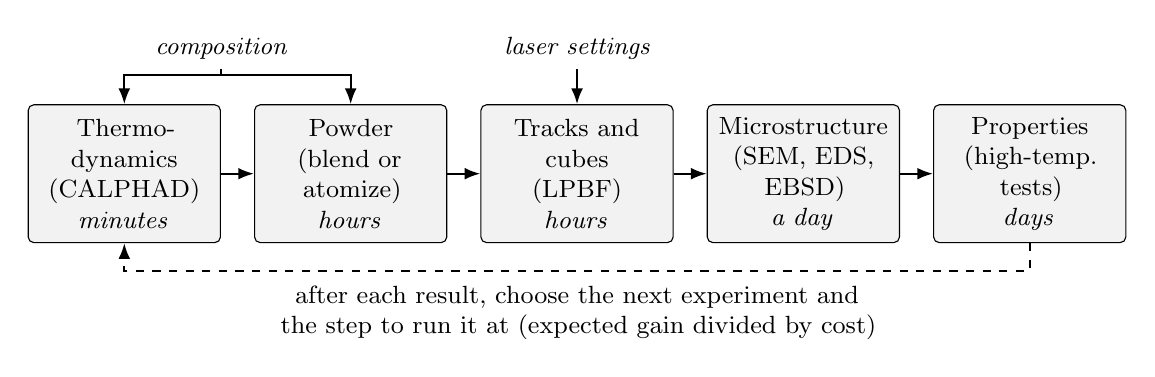
\begin{tikzpicture}[
  font=\small,
  node distance=0.42cm,
  box/.style={draw, rounded corners=2pt, fill=black!5, align=center,
    text width=2.3cm, minimum height=1.75cm, inner sep=2pt},
  arr/.style={-{Latex[length=2mm]}, thick},
  input/.style={font=\small\itshape, align=center}
]
\node[box] (s1) {Thermo-\\dynamics\\(CALPHAD)\\\textit{minutes}};
\node[box, right=of s1] (s2) {Powder\\(blend or\\atomize)\\\textit{hours}};
\node[box, right=of s2] (s3) {Tracks and\\cubes\\(LPBF)\\\textit{hours}};
\node[box, right=of s3] (s4) {Microstructure\\(SEM, EDS,\\EBSD)\\\textit{a day}};
\node[box, right=of s4] (s5) {Properties\\(high-temp.\\tests)\\\textit{days}};
\foreach \a/\b in {s1/s2, s2/s3, s3/s4, s4/s5} \draw[arr] (\a) -- (\b);
\node[input, above=0.45cm of s1.north east] (comp) {composition};
\draw[arr] (comp.south) -- ++(0,-0.08) -| (s1.north);
\draw[arr] (comp.south) -- ++(0,-0.08) -| (s2.north);
\node[input, above=0.45cm of s3] (laser) {laser settings};
\draw[arr] (laser) -- (s3);
\draw[arr, dashed] (s5.south) -- ++(0,-0.35) -| (s1.south);
\node[below=0.42cm of s3.south, align=center, text width=13cm]
  {after each result, choose the next experiment and the step to run it at
  (expected gain divided by cost)};
\end{tikzpicture}
\caption{The workflow as a network of linked models. Each step has its own
model that predicts the outputs of that step with uncertainty. Typical costs
are shown in italics.}
\label{fig:network}
\end{figure}

\subsection{Approach}
Our ultrasonic atomizer (AMAZEMET rePOWDER) has an induction-melting module,
which is limited to alloys that melt below about 1300~\degC. It covers
aluminum alloys like those in our preliminary work. Refractory alloys need its
plasma-arc melting module, which we will request separately through the
Defense University Research Instrumentation Program (DURIP) and which is not
part of this request. In this project, refractory compositions will be made by
blending elemental and master-alloy powders that the laser melts and mixes
during printing (in situ alloying), a route already used to make refractory
high-entropy alloys by laser deposition~\cite{dobbelstein2019}. Blending lets
us change composition by weighing powders, without a new atomization run for
each alloy. It also makes mixing in the melt pool part of the synthesis
problem, since laser power, scan path, and the number of remelting passes
control how fully the high-melting elements dissolve~\cite{yeung2026}. If the
plasma module is funded, pre-alloyed refractory powders made by ultrasonic
atomization, as recently shown for TiZrNbHfTa~\cite{dodge2026}, will be added
as a second synthesis route and compared with the blended route.

Each round, the platform will choose compositions and laser settings (power,
scan speed, hatch spacing, and remelting passes) for the next experiments. The
early measurements are single laser tracks, which show melt-pool size,
balling, and cracking, and small cubes, which give density and porosity.
Selected cubes will be sectioned and examined by scanning electron microscopy
(SEM), by energy-dispersive X-ray spectroscopy (EDS) for chemical uniformity
and unmelted particles, and by electron backscatter diffraction (EBSD) for
grain size, shape, and texture. The most promising candidates will be tested
mechanically at high temperature, with hardness as a cheaper stand-in.

The platform will decide what to run next with the cost-aware method of
Buathong et al.~\cite{buathong2024}. For each possible experiment, it
estimates how much the result is expected to improve the search, divides that
by the cost of the experiment, and runs the best one. To our knowledge, no prior
work has used this kind of cost-aware search to decide which step of a
physical alloy additive manufacturing workflow (powder production, printing,
microstructure, or property testing) to run next. Recent closed-loop campaigns
on additively manufactured alloys instead optimize composition with a single
model and a fixed set of measurements~\cite{talbot2026}.

\subsection{Data, measurements, and analysis}
Targets will be stated as microstructure descriptors computed from the SEM,
EDS, and EBSD maps: relative density, crack density, a chemical-uniformity
index (the spread of local composition across an EDS map), grain size and
aspect ratio, and texture strength. A target microstructure is then a region
in this descriptor space, and the network will report the probability that a
candidate lands in it. Replicate tracks and cubes at fixed settings will
measure build-to-build scatter. The models will treat this scatter as noise
that more data cannot remove and keep it separate from model uncertainty,
which shrinks as data accumulate, so the predicted probability reflects both.
Calibration will be checked on held-out builds by comparing predicted
probabilities with observed success rates, and the value of the early
measurements will be tested by fitting models with and without them. The
cost-aware search will be compared on equal budgets with random selection and
with standard Bayesian optimization over the full chain, first in
retrospective benchmarks built from our own data and then in live campaigns.

\subsection{Benchmarks and Gold Standard Science}
Progress will be measured against benchmarks fixed before the campaigns
start. For H1, predicted probabilities should fall within 10 percentage points
of observed success rates on held-out builds. For H2, the cost-aware search
should reach the target microstructure at no more than half the experimental
cost of the full-chain baseline. Data, code, and models will be released each
year, and results that reject a hypothesis will be published like any other
result. The work will follow the Gold Standard Science tenets in NOFO
Section C.3, with reproducible and transparent methods, stated uncertainty,
falsifiable hypotheses, and unbiased peer review.

\section{Potential team members and development plan}

The project is a single-investigator effort with no collaborators or
subawards. The PI will lead the work and supervise one Ph.D. student, funded
for three years, who will run the LPBF and characterization campaigns, and two
part-time undergraduate researchers, who will prepare powder blends and
specimens. LPBF builds will be bought from a University of Utah user
facility at \$800 per build. All other work will use BYU facilities: the
powder metallurgy laboratory of the PI with the ultrasonic atomizer, the BYU
Microscopy Center for SEM, EDS, and EBSD, and BYU high-performance computing
for CALPHAD.

Year~1 will build the linked models from CALPHAD calculations and the aluminum
data already in hand, commission in situ alloying of refractory powder blends,
run replicated single-track and cube campaigns to measure scatter, and
assemble the retrospective benchmark. Year~2 will run closed-loop campaigns on
RCCAs in the Mo-Nb-Ta-W-Hf-Zr-Ti system toward target microstructures, add the
EBSD-based descriptors and high-temperature tests, and test H1 on held-out
builds. Year~3 will test H2 in live campaigns against the full-chain baseline,
carry the method to the nickel superalloys to test transfer, and release the
software and data. The award would establish a research program at BYU on
synthesis by design for extreme-environment alloys. Results will be
presented at AFOSR program reviews and at TMS and MS\&T meetings.

\section{Preliminary results and PI qualifications}

Since the lab started at BYU in December 2025, we have implemented the
multi-fidelity Bayesian optimization method described above and set up a
working CALPHAD workflow on BYU high-performance computing. We have also
completed a powder-to-part demonstration on a baseline aluminum alloy, with
atomized powder, LPBF builds, SEM and EDS results, and tensile data in hand.
We collected these data to vet the workflow and reduce its risk before
refractory alloys are attempted.

The PI has worked across Bayesian optimization, autonomous laboratories, and
microstructure science. The PI developed Honegumi, an interface that helps
experimentalists set up Bayesian optimization, and consulted on the 1.0 release
of the Ax optimization platform from Meta. The PI co-authored the
\emph{Chemical Reviews} survey of self-driving laboratories, writing its
structural-materials section, and built the development laboratory of the
Acceleration Consortium at the University of Toronto. Earlier work inferred grain-boundary structure-property
models with propagated uncertainty, measured the accuracy limits of EBSD-based
grain-boundary analysis, and included the design of a semi-automated
2500~\degC{} induction furnace for high-purity processing. The PI supervises
eight undergraduate researchers at BYU. All publications and presentations are
listed in the attached curriculum vitae.

% ===========================================================================
% References (excluded from the 5-page limit)
% ===========================================================================
\clearpage
\setcounter{page}{1}
\renewcommand{\thepage}{R\arabic{page}}  % keep reference pages out of 1-5
\begin{thebibliography}{99}
\setlength{\itemsep}{2pt}

\bibitem{pollock2006}
T.~M. Pollock and S.~Tin, ``Nickel-based superalloys for advanced turbine
engines: chemistry, microstructure and properties,'' \emph{J. Propul. Power}
\textbf{22}(2), 361--374 (2006).
\href{https://doi.org/10.2514/1.18239}{doi:10.2514/1.18239}

\bibitem{peters2024}
A.~B. Peters, D.~Zhang, S.~Chen, C.~Ott, C.~Oses, S.~Curtarolo, I.~McCue,
T.~M. Pollock, and S.~Eswarappa Prameela, ``Materials design for hypersonics,''
\emph{Nat. Commun.} \textbf{15}, 3328 (2024).
\href{https://doi.org/10.1038/s41467-024-46753-3}{doi:10.1038/s41467-024-46753-3}

\bibitem{senkov2018}
O.~N. Senkov, D.~B. Miracle, K.~J. Chaput, and J.-P. Couzinie, ``Development
and exploration of refractory high entropy alloys---A review,''
\emph{J. Mater. Res.} \textbf{33}(19), 3092--3128 (2018).
\href{https://doi.org/10.1557/jmr.2018.153}{doi:10.1557/jmr.2018.153}

\bibitem{debroy2018}
T.~DebRoy, H.~L. Wei, J.~S. Zuback, T.~Mukherjee, J.~W. Elmer,
J.~O. Milewski, A.~M. Beese, A.~Wilson-Heid, A.~De, and W.~Zhang, ``Additive
manufacturing of metallic components -- Process, structure and properties,''
\emph{Prog. Mater. Sci.} \textbf{92}, 112--224 (2018).
\href{https://doi.org/10.1016/j.pmatsci.2017.10.001}{doi:10.1016/j.pmatsci.2017.10.001}

\bibitem{usgs2026}
U.S. Geological Survey, \emph{Mineral Commodity Summaries 2026}, ver.~1.3
(2026), pp.~70, 156.
\href{https://doi.org/10.3133/mcs2026}{doi:10.3133/mcs2026}

\bibitem{campo2026}
E.~M. Campo, R.~J. Hanisch, and J.~C. Agar, ``From discovery to deployment:
A national AI strategy for materials readiness across energy and defense,''
\emph{MRS Bull.} (2026), published online 23 Sep 2026.
\href{https://doi.org/10.1557/s43577-026-01181-0}{doi:10.1557/s43577-026-01181-0}

\bibitem{andersson2002}
J.-O. Andersson, T.~Helander, L.~H{\"o}glund, P.~Shi, and B.~Sundman,
``Thermo-Calc \& DICTRA, computational tools for materials science,''
\emph{Calphad} \textbf{26}(2), 273--312 (2002).
\href{https://doi.org/10.1016/S0364-5916(02)00037-8}{doi:10.1016/S0364-5916(02)00037-8}

\bibitem{otis2017}
R.~Otis and Z.-K. Liu, ``pycalphad: CALPHAD-based computational thermodynamics
in Python,'' \emph{J. Open Res. Softw.} \textbf{5}(1), 1 (2017).
\href{https://doi.org/10.5334/jors.140}{doi:10.5334/jors.140}

\bibitem{astudillo2021}
R.~Astudillo and P.~I. Frazier, ``Bayesian optimization of function networks,''
\emph{Advances in Neural Information Processing Systems} \textbf{34},
14463--14475 (2021).
\href{https://proceedings.neurips.cc/paper_files/paper/2021/hash/792c7b5aae4a79e78aaeda80516ae2ac-Abstract.html}{NeurIPS proceedings},
\href{https://arxiv.org/abs/2112.15311}{arXiv:2112.15311}

\bibitem{buathong2024}
P.~Buathong, J.~Wan, R.~Astudillo, S.~Daulton, M.~Balandat, and P.~I. Frazier,
``Bayesian optimization of function networks with partial evaluations,''
\emph{Proc. 41st Int. Conf. Machine Learning (ICML)}, PMLR \textbf{235},
4752--4784 (2024).
\href{https://proceedings.mlr.press/v235/buathong24a.html}{PMLR proceedings},
\href{https://arxiv.org/abs/2311.02146}{arXiv:2311.02146}

\bibitem{dobbelstein2019}
H.~Dobbelstein, E.~L. Gurevich, E.~P. George, A.~Ostendorf, and
G.~Laplanche, ``Laser metal deposition of compositionally graded TiZrNbTa
refractory high-entropy alloys using elemental powder blends,''
\emph{Addit. Manuf.} \textbf{25}, 252--262 (2019).
\href{https://doi.org/10.1016/j.addma.2018.10.042}{doi:10.1016/j.addma.2018.10.042}

\bibitem{yeung2026}
H.~Yeung, J.~Weaver, A.~Ponsot, J.~Dar, Y.~Zhang, D.~Lin, A.~Chuang,
M.~C. Gao, and F.~Zhang, ``Laser stirring with elliptical scanning enables
on-demand alloying in additive manufacturing,'' \emph{Addit. Manuf.}
\textbf{118}, 105101 (2026).
\href{https://doi.org/10.1016/j.addma.2026.105101}{doi:10.1016/j.addma.2026.105101}

\bibitem{dodge2026}
B.~S. Dodge, S.~Niraula, N.~Shokri, J.~D. Gillham, and T.~A. Berfield,
``Ultrasonic atomization of a refractory high-entropy alloy TiZrNbHfTa for
additive manufacturing,'' \emph{Powders} \textbf{5}(3), 25 (2026).
\href{https://doi.org/10.3390/powders5030025}{doi:10.3390/powders5030025}

\bibitem{talbot2026}
A.~Talbot, S.~S. Dash, J.~Li, C.~Cheng, M.~Ramesh, X.~Shang, J.~Zhang,
C.~Cojocaru, J.~Hattrick-Simpers, and Y.~Zou, ``Active learning for the
accelerated discovery of complex concentrated NiCoCr alloys in additive
manufacturing,'' \emph{npj Adv. Manuf.} (2026), published online 23 Jun 2026.
\href{https://doi.org/10.1038/s44334-026-00098-5}{doi:10.1038/s44334-026-00098-5}

\end{thebibliography}

% ===========================================================================
% Curriculum vitae (excluded from the 5-page limit; NOFO: "All publications
% and presentations must be identified")
% ===========================================================================
\IfFileExists{../bios/baird-CV.pdf}{%
  \includepdf[pages=-,pagecommand={\thispagestyle{empty}}]{../bios/baird-CV.pdf}%
}{}

\end{document}
